% Vietnamese translation for OI Public Library
% Source-PDF: IOI中国国家候选队论文/2004/肖天.pdf
\documentclass[11pt]{article}
\usepackage{oipl-vn}
\usepackage{tikz}
\usetikzlibrary{arrows.meta,positioning}

\title{Tư tưởng đồ thị phân tầng và ứng dụng trong thi tin học}
\author{Xiao Tian}
\date{}

\begin{document}
\maketitle

\origtitle{Layered graph thinking and its applications in informatics contests}
\sourcepath{IOI China candidate team papers / 2004 / Xiao Tian.pdf}

\section*{Tóm tắt}

Thông qua lời giải của một số bài toán trong thi tin học, bài viết đưa ra một
tư tưởng mô hình hóa để giải bài: \term{tư tưởng đồ thị phân tầng}. Tư tưởng
này khai thác tính chất của bài toán, sao chép đồ thị trừu tượng hóa từ bài
toán ban đầu thành nhiều tầng rồi nối chúng thành một đồ thị lớn hơn. Nhờ đó,
một mô hình đồ thị vốn khó diễn đạt bằng ngôn ngữ toán học chặt chẽ trở nên
gọn gàng và nghiêm ngặt hơn, tạo nền tảng tốt cho bước giải tiếp theo.

\paragraph{Từ khóa.}
Đồ thị phân tầng; lý thuyết đồ thị; mô hình toán học; đường đi ngắn nhất; thi
tin học.

\section{Mở đầu}

Khi dùng máy tính để giải một bài toán thực tế, về bản chất ta phải nói thật
chi tiết cho máy tính biết cần làm gì, để từ dữ liệu vào do con người cung cấp
nó sinh ra kết quả mong muốn. Vì máy tính thông thường chỉ xử lý được tín hiệu
số, bài toán thực tế phải được chuyển thành bài toán toán học thì máy tính mới
có thể giúp ta. Bước chuyển đó chính là xây dựng mô hình toán học.

Việc xây dựng mô hình toán học rất quan trọng trong quá trình giải bài bằng
máy tính. Nó chuyển hóa những vấn đề máy tính không hiểu được, lượng hóa mọi
sự vật, rồi cuối cùng biến bài toán thành một quá trình chỉ còn chứa thao tác
toán học. Đó là cây cầu nối giữa tư duy con người và máy tính. Hơn nữa, chất
lượng của mô hình toán học ảnh hưởng trực tiếp đến việc trao đổi thông tin
giữa người và máy, cũng như ảnh hưởng đến cách máy tính ``hiểu'' bài toán.
Một mô hình tốt nắm được bản chất bài toán, diễn đạt ngắn gọn rõ ràng, giúp
con người dễ tìm ra phương pháp hiệu quả và truyền phương pháp đó cho máy
tính qua chương trình. Ngược lại, với cùng một bài toán, nếu mô hình không
nắm được bản chất, ta có thể không giải nổi bài, hoặc không tìm được cách làm
hiệu quả, càng không thể nói cho máy tính biết phải làm thế nào.

Vì mục đích của mô hình hóa là giải bài, người ta thường mong muốn quy bài
toán về một bài toán kinh điển đã được giải tốt, hoặc về một tổ hợp hữu cơ của
một số bài toán như vậy. Khi đó chỉ cần áp dụng những thành quả đã có. Chẳng
hạn, sắp xếp, đường đi ngắn nhất một nguồn, luồng mạng đều là các bài toán
kinh điển: không chỉ có thuật toán tổng quát, mà các trường hợp đặc biệt và
biến thể cũng đã được nghiên cứu sâu.

Tuy nhiên mọi chuyện không phải lúc nào cũng như ta mong muốn. Có những bài
toán về cơ bản có thể quy về bài toán đã biết, nhưng sau khi thêm một vài yếu
tố gây nhiễu, tính chất ban đầu thay đổi, khiến mô hình toán học cũ khó còn
được diễn đạt bằng ngôn ngữ chặt chẽ. Một phần các bài toán đồ thị kiểu này
có thể được xử lý bằng tư tưởng đồ thị phân tầng được trình bày trong bài
viết này.

Tư tưởng này chú trọng khai thác tính chất của bài toán ban đầu. Bằng cách mở
rộng mô hình toán học của bài toán, ta đưa các yếu tố gây nhiễu vào mô hình
mới, khôi phục tính chặt chẽ của mô hình, rồi liên hệ nó với những bài toán
đã giải được để thu được thuật toán hiệu quả.

\section{Đưa ra tư tưởng đồ thị phân tầng}

\subsection{Lời giải cho một bài toán}

\paragraph{Ví dụ 1: Cứu binh nhì Ryan.}
Cho một mê cung hình chữ nhật gồm $N$ hàng và $M$ cột, tổng cộng $N M$ ô. Hai
ô kề cạnh có thể thông nhau, hoặc giữa chúng có một cánh cửa khóa, hoặc giữa
chúng có một bức tường không thể vượt qua. Một số ô trong mê cung chứa chìa
khóa. Tất cả các cửa được chia thành $P$ loại; các cửa cùng loại dùng chung
một loại chìa khóa, các loại cửa khác nhau dùng chìa khóa khác nhau.

Yêu cầu đi từ góc trên trái đến góc dưới phải để cứu binh nhì Ryan. Mỗi lần
di chuyển từ một ô sang ô kề cạnh tính là một bước. Chỉ khi đã lấy chìa khóa
tương ứng mới có thể mở cửa thuộc loại đó. Hãy tìm số bước ít nhất.

Cách giải chuẩn của bài này là quy hoạch động theo tập loại chìa khóa đã có,
với độ phức tạp thời gian $O(2^P N^2)$ trong trường hợp mê cung có kích thước
cùng bậc. Thực ra thuật toán đó có thể được giải thích ngắn gọn hơn bằng tư
tưởng đồ thị phân tầng.

Trước hết bỏ qua chìa khóa và cửa. Khi đó bài toán chỉ là tìm một đường đi
ngắn nhất trong một đồ thị ẩn cho trước. Mô hình toán học rất đơn giản: cho
đồ thị $G$, trong đó mỗi đỉnh tương ứng với một ô của bản đồ. Khi và chỉ khi
hai ô kề nhau và giữa chúng không có tường, hai đỉnh tương ứng được nối bởi
một cạnh. Ta cần tìm độ dài đường đi ngắn nhất từ đỉnh tương ứng với góc trên
trái đến đỉnh tương ứng với góc dưới phải.

\begin{center}
\begin{tikzpicture}[scale=0.72, every node/.style={font=\small}]
  \draw[step=1cm, gray!45] (0,0) grid (5,4);
  \draw[line width=1.2pt] (0,0) rectangle (5,4);
  \draw[line width=1.2pt] (1,0) -- (1,2) -- (3,2) -- (3,4);
  \draw[line width=1.2pt] (2,1) -- (4,1) -- (4,3);
  \node at (0.5,3.5) {$S$};
  \node at (4.5,0.5) {$T$};
  \node at (1.5,2.5) {$k_1$};
  \node at (3.5,2.5) {$k_2$};
  \node at (2.5,0.5) {$d_1$};
  \node at (4.5,1.5) {$d_2$};
  \begin{scope}[xshift=7cm]
    \foreach \x in {0,...,4}
      \foreach \y in {0,...,3}
        \fill (\x,\y) circle (1.8pt);
    \foreach \x in {0,...,3}
      \foreach \y in {0,...,3}
        \draw[gray!60] (\x,\y) -- (\x+1,\y);
    \foreach \x in {0,...,4}
      \foreach \y in {0,...,2}
        \draw[gray!60] (\x,\y) -- (\x,\y+1);
    \node at (2,-0.7) {đồ thị ô khi bỏ qua cửa};
  \end{scope}
\end{tikzpicture}
\end{center}

Khi thêm yếu tố chìa khóa và cửa, đường đi ngắn nhất cần tìm có thêm ràng
buộc: chỉ sau khi đến ô có chìa khóa mới có thể đi qua cửa tương ứng. Nói
cách khác, một số cạnh trong đồ thị chỉ đi được khi thỏa điều kiện. Vì vậy ta
không thể chỉ tìm đường đi ngắn nhất đơn giản, mà phải xét thời điểm nào cạnh
đó đi được, thời điểm nào không đi được. Điều này buộc ta ghi nhận những loại
chìa khóa đã lấy.

Ta cải tạo mô hình ban đầu như sau. Sao chép đồ thị $G$ thành $2^P$ bản, ký
hiệu
\[
  G(s_1,s_2,\ldots,s_P),
\]
trong đó $s_i=0$ nghĩa là chưa có chìa khóa loại $i$, còn $s_i=1$ nghĩa là đã
có chìa khóa loại $i$, với $i=1,2,\ldots,P$. Trong mỗi đồ thị
$G(s_1,s_2,\ldots,s_P)$, nếu $s_i=0$ thì xóa mọi cạnh tương ứng với cửa loại
$i$, vì khi chưa có chìa khóa loại đó thì không thể đi qua các cửa đó. Các
cạnh còn lại được đổi thành cung hai chiều có trọng số $1$.

Với mọi cặp đỉnh $(u,v)$ và số nguyên $i$, nếu
\begin{itemize}
  \item $u$ thuộc tầng $G(s_1,\ldots,s_{i-1},0,s_{i+1},\ldots,s_P)$, còn $v$
  thuộc tầng $G(s_1,\ldots,s_{i-1},1,s_{i+1},\ldots,s_P)$, và cả hai cùng
  tương ứng với ô $(x,y)$;
  \item ô $(x,y)$ chứa chìa khóa loại $i$,
\end{itemize}
thì thêm cung có hướng $u\to v$ với trọng số $0$. Cung này biểu diễn rằng khi
đi đến ô $(x,y)$ ta có thể chuyển từ trạng thái chưa có chìa khóa loại $i$
sang trạng thái đã có chìa khóa loại $i$, không tốn thêm bước.

Như vậy, $2^P$ bản sao được nối thành một đồ thị có hướng gồm $2^P$ tầng.
Bài toán chuyển thành tìm giá trị nhỏ nhất trong các độ dài đường đi ngắn
nhất từ đỉnh góc trên trái ở tầng $G(0,0,\ldots,0)$ đến đỉnh góc dưới phải ở
mỗi tầng. Cần chú ý rằng đích không nhất thiết phải nằm ở tầng
$G(1,1,\ldots,1)$, vì cứu được binh nhì Ryan có thể không cần lấy đủ mọi loại
chìa khóa.

\begin{center}
\begin{tikzpicture}[scale=0.78, node distance=1.4cm, every node/.style={font=\small}]
  \foreach \x/\y/\name in {0/2/A,3/2/B,0/0/C,3/0/D} {
    \begin{scope}[shift={(\x,\y)}]
      \draw[gray!50] (0,0) rectangle (2,1.2);
      \node at (1,0.6) {$G_{\name}$};
      \fill (0.35,0.9) circle (1.5pt);
      \fill (1.65,0.25) circle (1.5pt);
    \end{scope}
  }
  \draw[-{Stealth[length=2.2mm]}] (1,2.6) -- (4,2.6);
  \draw[-{Stealth[length=2.2mm]}] (1,2.6) -- (1,0.6);
  \draw[-{Stealth[length=2.2mm]}] (4,2.6) -- (4,0.6);
  \draw[-{Stealth[length=2.2mm]}] (1,0.6) -- (4,0.6);
  \node at (2.5,-0.55) {các cung trọng số $0$ nối giữa những tầng khác trạng thái chìa khóa};
\end{tikzpicture}
\end{center}

\subsection{Tiểu kết}

Có thể thấy, dùng tư tưởng này ta xây dựng được một mô hình toán học gọn gàng
và chặt chẽ hơn, từ đó dễ thu được thuật toán hiệu quả. Điều quan trọng là đồ
thị mới có một số tính chất tốt.

Thứ nhất, các tầng được sinh ra bằng cách sao chép, nên mọi tầng rất giống
nhau. Trong chương trình ta chỉ cần phân biệt khái niệm tầng về mặt logic,
không cần thật sự lưu thêm các tầng mới, thậm chí gần như không tốn thời gian
xử lý riêng cho chúng.

Thứ hai, vì các tầng tương tự nhau, nhiều kết quả tính toán là giống nhau.
Ta chỉ cần tính những kết quả đó một lần rồi lưu lại, thay vì tính đi tính
lại. Nhìn bề ngoài đồ thị lớn hơn, nhưng về thực chất quy mô bài toán không
tăng tương ứng.

Thứ ba, giữa các tầng có thứ tự tô pô. Điều này có nghĩa là các xử lý như
truy hồi giữa các tầng có thể được thực hiện dễ dàng, tạo nền tảng tốt để
tìm thuật toán hiệu quả.

Trong lời giải của ví dụ 1, các đặc điểm trên chưa thể hiện rõ, nên thuật
toán được nêu không tốt hơn thuật toán chuẩn. Nhưng những đặc điểm đó cho
thấy tư tưởng đồ thị phân tầng vẫn có nhiều tiềm năng; đặc biệt, việc các
tầng có nhiều kết quả tính chung có thể loại bỏ đáng kể phép tính dư thừa và
hạ độ phức tạp thời gian. Ví dụ tiếp theo sẽ cho thấy điều này.

\section{Ứng dụng của tư tưởng đồ thị phân tầng}

\paragraph{Ví dụ 2: Cải tạo mê cung.}
Cho một mê cung hình chữ nhật được chia thành $N$ hàng theo hướng bắc--nam và
$M$ cột theo hướng đông--tây, tổng cộng $N M$ ô. Vị trí một ô được biểu diễn
bằng cặp có thứ tự gồm số hàng và số cột. Giữa hai ô kề nhau theo hướng
bắc--nam hoặc đông--tây có thể có tường, cũng có thể không có tường; tường là
không thể vượt qua.

Giả sử có $P$ người, lần lượt xuất phát từ $P$ điểm bắt đầu cho trước. Họ chỉ
được đi về phía nam hoặc phía đông và phải lần lượt đến $P$ điểm kết thúc cho
trước. Hỏi ít nhất phải phá bao nhiêu bức tường để việc này khả thi, tức mọi
người đều có thể đi từ điểm xuất phát của mình đến điểm kết thúc của mình
theo đúng luật. Các tham số thỏa
\[
  3\le N,M\le 20,\qquad 1\le P\le 3.
\]

Để tiện trình bày, dưới đây chỉ xét trường hợp $M=N$ và $P=3$. Khi $P<3$, có
thể thêm những người có điểm xuất phát trùng điểm kết thúc để đưa $P$ lên
$3$.

\subsection{Cách giải 1: quy hoạch động giống bài lấy số trên ô vuông}

Chia giai đoạn bằng các đường thẳng song song với đường chéo phụ. Gọi
$S(i,x_1,x_2,x_3)$ là số tường ít nhất cần phá khi ba người lần lượt đi đến
hàng $x_1,x_2,x_3$ trên đường chéo thứ $i$. Với mỗi trạng thái, mỗi người có
hai cách đi là về nam hoặc về đông, tổng cộng $2^3=8$ quyết định. Công thức
chuyển trạng thái có dạng
\[
\begin{aligned}
S(i,x_1,x_2,x_3)=\min\{&
S(i-1,x_1-1,x_2-1,x_3-1)+\delta_{111},\\
&S(i-1,x_1-1,x_2-1,x_3)+\delta_{110},\\
&S(i-1,x_1-1,x_2,x_3-1)+\delta_{101},\\
&S(i-1,x_1-1,x_2,x_3)+\delta_{100},\\
&S(i-1,x_1,x_2-1,x_3-1)+\delta_{011},\\
&S(i-1,x_1,x_2-1,x_3)+\delta_{010},\\
&S(i-1,x_1,x_2,x_3-1)+\delta_{001},\\
&S(i-1,x_1,x_2,x_3)+\delta_{000}\}.
\end{aligned}
\]
Ở đây mỗi $\delta$ biểu diễn số tường cần phá ứng với quyết định đó, hiển
nhiên chỉ có thể nhận giá trị trong $\{0,1,2,3\}$. Các trường hợp nhỏ được xử
lý theo cùng nguyên tắc. Ngoài ra, vì điểm xuất phát của mỗi người không
nhất thiết là góc trên trái và điểm kết thúc cũng không nhất thiết là góc dưới
phải, khi truy hồi còn phải xử lý thêm một số chi tiết biên. Độ phức tạp thời
gian của thuật toán này là $O(N^4)$.

\subsection{Cách giải 2: dùng đồ thị phân tầng để chuyển thành đường đi ngắn nhất}

Trước hết phân tích đặc điểm của bài toán. Tính khả thi của tuyến đường của
mỗi người không bị các thành viên khác ảnh hưởng; khi tính chi phí, những
người khác nhau chỉ liên hệ với nhau nếu họ đi qua cùng một bức tường. Nếu bỏ
qua quan hệ này, tuyến đường của mỗi người phải là một đường đi ngắn nhất giữa
điểm xuất phát và điểm kết thúc của người đó. Nói cách khác, có người có thể
phải nhường theo người khác nên tuyến đường của họ không phải ngắn nhất,
nhưng trên những đoạn không chung, tuyến đường của mỗi thành viên đều có tính
chất đường đi ngắn nhất.

\paragraph{Định nghĩa 1.}
Một \term{đoạn thuần} là một phần của một nghiệm khả thi sao cho giao của nó
với tuyến đường của mỗi thành viên hoặc rỗng, hoặc chính là toàn bộ đoạn đó
tức đoạn đó là một phần tuyến đường của thành viên ấy. Trực quan mà nói, đoạn
thuần trong một nghiệm khả thi không phân nhánh.

\paragraph{Định nghĩa 2.}
Một \term{đoạn thuần cực đại} là một đoạn thuần của một nghiệm, nhưng không
phải là đoạn con của bất kỳ đoạn thuần nào khác trong cùng nghiệm đó.

Khi đó tính chất vừa nêu có thể phát biểu như sau: mọi đoạn thuần trong một
nghiệm tối ưu đều là đường đi ngắn nhất nối hai đầu mút của nó. Vì vậy, một
nghiệm tối ưu có thể được xác định duy nhất bởi tập các đầu mút của mọi đoạn
thuần cực đại. Điều này cho ta một thuật toán thô sơ: liệt kê các đầu mút
đó. Dù độ phức tạp của thuật toán này không chấp nhận được, nó gợi ra hướng
tận dụng đầy đủ tính chất đường đi ngắn nhất của các đoạn thuần.

Tiếp tục khai thác đặc điểm bài toán. Khác biệt lớn nhất giữa bài này và bài
toán đường đi ngắn nhất thông thường là có nhiều người; khi họ có đoạn đường
chung, trọng số của đoạn chung chỉ được tính một lần. Do đó nắm được cấu trúc
của các đoạn chung là điểm then chốt.

\paragraph{Định lý 1.}
Tồn tại một nghiệm tối ưu trong đó đoạn chung của hai người bất kỳ không quá
một đoạn; nói cách khác, hai tuyến đường bất kỳ sẽ không gặp nhau, tách ra,
rồi lại gặp nhau lần nữa.

\paragraph{Chứng minh.}
Giả sử trong một nghiệm tối ưu $T$ có hai người $A,B$ tách nhau tại điểm $P$
rồi lại gặp nhau tại điểm $Q$. Gọi trọng số hai tuyến đường của họ giữa $P$
và $Q$ lần lượt là $W_A,W_B$. Khi đó tổng chi phí của $A,B$ trên đoạn
$P,Q$ là
\[
  W=W_A+W_B.
\]
Rõ ràng tồn tại một nghiệm khả thi khác $T'$, chỉ khác $T$ ở chỗ tuyến đường
của $B$ giữa $P$ và $Q$ được đổi thành giống tuyến đường của $A$. Khi đó tổng
chi phí của $A,B$ trên đoạn $P,Q$ trong $T'$ là $W'=W_A$. Vì $W'\le W$, nên
$T'$ cũng là nghiệm tối ưu. Bằng hữu hạn lần biến đổi như vậy, ta loại bỏ
được mọi tình huống ``gặp nhau, tách ra, rồi lại gặp nhau'' trong một nghiệm
tối ưu mà vẫn giữ tính tối ưu.

\paragraph{Định lý 2.}
Khi $P\le 3$, tồn tại một nghiệm tối ưu sao cho hợp của mọi tuyến đường không
có chu trình, nếu xem các tuyến đường là đường đi vô hướng.

\paragraph{Chứng minh.}
Đây thực chất là một mở rộng đơn giản của định lý 1. Giả sử một nghiệm tối ưu
$T$ có chu trình, và sau khi dùng định lý 1 để loại bỏ chu trình do hai người
tạo ra thì vẫn còn chu trình. Khi đó chu trình ấy tất yếu do ba người tạo ra,
và chỉ có dạng như sơ đồ dưới đây. Tương tự chứng minh của định lý 1, đoạn
$PS$ của người $C$ có thể được thay bằng $PQRS$, qua đó bỏ chi phí của đoạn
$PS$; nghiệm mới thu được vẫn là tối ưu. Vì vậy luôn có thể thu được một
nghiệm tối ưu không chu trình.

\begin{center}
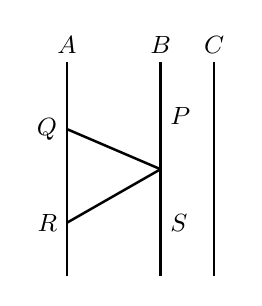
\begin{tikzpicture}[scale=0.85, every node/.style={font=\small}]
  \draw[line width=0.9pt] (0,0) -- (0,3.2);
  \draw[line width=0.9pt] (1.4,0) -- (1.4,3.2);
  \draw[line width=0.9pt] (2.2,0) -- (2.2,3.2);
  \draw[line width=0.9pt] (0,0.8) -- (1.4,1.6) -- (1.4,2.4);
  \draw[line width=0.9pt] (0,2.2) -- (1.4,1.6) -- (1.4,0.8);
  \node[left] at (0,2.2) {$Q$};
  \node[left] at (0,0.8) {$R$};
  \node[right] at (1.4,2.4) {$P$};
  \node[right] at (1.4,0.8) {$S$};
  \node at (0,3.45) {$A$};
  \node at (1.4,3.45) {$B$};
  \node at (2.2,3.45) {$C$};
\end{tikzpicture}
\end{center}

\paragraph{Định lý 3.}
Khi $P\le 3$, với một nghiệm tối ưu không chu trình $T$, tất cả các đoạn chung
trong $T$ có thể được phủ bởi một tuyến đường từ góc trên trái đến góc dưới
phải.

\paragraph{Chứng minh.}
Giả sử trong $T$ có hai đoạn chung không thể được phủ bởi một tuyến đường giả
tưởng từ góc trên trái đến góc dưới phải. Khi đó rõ ràng chúng không thể
thuộc cùng một tuyến đường của một người, vì nếu không tuyến đường của người
đó đã thỏa yêu cầu. Mặt khác, mỗi đoạn chung thuộc ít nhất hai người, nên
phải có $P\ge 4$, mâu thuẫn với $P\le 3$.

\paragraph{Định nghĩa.}
Với một nghiệm tối ưu $T$, nếu một tuyến đường từ góc trên trái đến góc dưới
phải có thể phủ mọi đoạn chung trong $T$, ta gọi tuyến đường đó là
\term{tuyến chính} của $T$.

Vậy một nghiệm tối ưu có thể được mô tả như sau: nó gồm một tuyến chính và
một số tuyến nhánh nối từ tuyến chính đến các điểm xuất phát và điểm kết thúc
của các thành viên. Trong nghiệm tối ưu này, mỗi thành viên xuất phát từ điểm
của mình; hoặc trước hết đi theo nhánh để vào tuyến chính, đi một đoạn trên
tuyến chính rồi lại đi theo nhánh đến đích, hoặc không đi qua tuyến chính mà
đi thẳng đến đích. Vì tuyến chính phủ mọi đoạn chung, mọi tuyến nhánh đều là
đoạn thuần và có tính chất đường đi ngắn nhất. Dùng tính chất này, ta có thể
tiền xử lý để tìm độ dài mọi tuyến nhánh, rồi xử lý giống trường hợp $P=1$
bằng quy hoạch động trong $O(N^2)$.

Vấn đề còn lại là xác định tuyến chính. Dễ thấy vấn đề này rất giống trường
hợp $P=1$, chỉ khác là đồng thời phải xác định các điểm tuyến nhánh nhập vào
và tách khỏi tuyến chính. Có thể xem việc một tuyến nhánh nhập vào hoặc tách
khỏi tuyến chính là sự thay đổi trạng thái của tuyến chính. Khi đó ta có thể
dùng tư tưởng phân tầng đồ thị để giải bài toán.

Vì quá trình đi từ điểm xuất phát đến điểm kết thúc của mỗi thành viên có thể
chia thành ba phần
\[
  \text{nhánh}\ \longrightarrow\ \text{tuyến chính}\ \longrightarrow\ \text{nhánh},
\]
nên đối với tuyến chính, mỗi thành viên có ba trạng thái:
\[
  0=\text{chưa vào},\qquad 1=\text{đang ở trên tuyến chính},\qquad
  2=\text{đã rời}.
\]
Với mỗi thành viên, ta sao chép bản đồ thành ba tầng; tổng cộng có $3^P$ tầng.
Ký hiệu $G(s_1,s_2,s_3)$ là tầng trong đó trạng thái của ba người là
$(s_1,s_2,s_3)$.

Xét thành viên 1. Từ mỗi đỉnh trong $G(0,s_2,s_3)$, ta nối một cung có hướng
đến đỉnh tương ứng trong $G(1,s_2,s_3)$; trọng số của cung là khoảng cách
ngắn nhất từ điểm xuất phát của thành viên 1 đến đỉnh đó, tức độ dài tuyến
nhánh đã được tính ở bước tiền xử lý. Nếu không thể đi từ điểm xuất phát của
thành viên 1 đến đỉnh đó, trọng số là $\infty$. Tương tự, từ mỗi đỉnh trong
$G(1,s_2,s_3)$, ta nối một cung có hướng đến đỉnh tương ứng trong
$G(2,s_2,s_3)$; trọng số là khoảng cách ngắn nhất từ đỉnh đó đến điểm kết thúc
của thành viên 1, hoặc $\infty$ nếu không đến được. Các thành viên khác được
xử lý tương tự.

Sau đó ta tìm đường đi ngắn nhất một nguồn từ đỉnh góc trên trái của tầng
$G(0,0,0)$ đến các đỉnh khác. Cần chú ý rằng đáp án không nhất thiết là độ
dài đường đi ngắn nhất từ góc trên trái của $G(0,0,0)$ đến góc dưới phải của
$G(2,2,2)$. Lý do là ở đây ta đã tạm bỏ qua tình huống đã nêu ở trên: một số
thành viên có thể không đi qua tuyến chính mà đi thẳng đến điểm kết thúc. Vì
vậy phải xét mỗi thành viên có vào tuyến chính hay không, tổng cộng $2^3=8$
trường hợp.

Đến đây bài toán đã được giải trọn vẹn. Trong cách giải 2, bước tiền xử lý
tốn $O(N^2)$, bước tìm đường đi ngắn nhất sau đó cũng tốn $O(N^2)$, nên tổng
độ phức tạp thời gian là $O(N^2)$, thấp hơn nhiều so với cách giải 1.

Tuy nhiên, cách giải 1 có thể mở rộng $P$ lên số lớn hơn, còn cách giải 2 chỉ
giải được trường hợp $P\le 3$. Trên thực tế, bài lấy số trên ô vuông đã nhắc
ở cách giải 1 có thể được giải tốt hơn bằng mô hình luồng mạng, nhưng tác giả
chưa xây dựng được mô hình luồng mạng cho bài mê cung này theo hướng đó. Đây
vẫn là một vấn đề có giá trị để tiếp tục nghiên cứu.

\section{Kết luận}

Khai thác tính chất bài toán là điểm then chốt của tư tưởng này. Đối với
những yếu tố mà ta chưa thể diễn đạt bằng ngôn ngữ toán học chặt chẽ, ta phân
tầng đồ thị, tương đương với việc phân loại các trường hợp, biến cái chưa
biết thành cái đã biết. Thực chất, cách làm này tăng cường những tính chất
vốn có của bài toán ban đầu. Sau xử lý đó, mô hình đồ thị mới có đặc trưng
nổi bật hơn và dễ tìm được phương pháp giải hơn.

\section*{Tài liệu tham khảo}

\begin{enumerate}
  \item Jiang Tao, Wang Yinghan, Luo Jingchen, \textit{Tuyển tập lời giải
  tinh chọn cho Olympic Tin học}, Nhà xuất bản Đại học Nam Kinh, 2000.6.
  \item Zhang Weixian, \textit{Phân tích đề thi Olympic Tin học thanh thiếu
  niên toàn quốc vòng khu vực, bậc trung học}, Nhà xuất bản Đại học Nam Kinh,
  2001.6.
\end{enumerate}

\appendix
\section{Đề bài Cải tạo mê cung}

Công ty giải trí XX gần đây giành được quyền sở hữu một số mê cung Hy Lạp cổ.
Để các mê cung cổ điển này thu hút thêm du khách, công ty muốn cải tạo chúng
một cách hợp lý. Nhiệm vụ của bạn là, dựa trên một mê cung đã cho và yêu cầu
của công ty, thiết kế một mê cung kiểu mới tốt nhất trên nền mê cung cũ.

Mê cung có dạng hình chữ nhật, được chia thành $N$ hàng theo hướng bắc--nam
và $M$ cột theo hướng đông--tây, tổng cộng $N M$ ô. Vị trí mỗi ô được biểu
diễn bằng cặp có thứ tự gồm số hàng và số cột. Giữa hai ô kề nhau theo hướng
bắc--nam hoặc đông--tây có một bức tường hoặc một cánh cửa. Tường không thể
vượt qua, còn cửa là hai chiều và có thể đi qua tùy ý. Để bảo vệ di tích,
công ty XX quyết định chỉ chuyển một số tường thành cửa, không thực hiện cải
tạo nào khác, và yêu cầu mê cung mới là tốt nhất, tức tổng số cửa mới phải ít
nhất.

Trước hết, công ty cần bạn thiết kế một mê cung tốt nhất sao cho du khách có
thể xuất phát từ bất kỳ ô nào trong mê cung mới sau cải tạo và đi đến bất kỳ
ô nào khác. Mê cung tốt nhất kiểu này được gọi là mê cung tốt nhất loại một,
chiếm $30\%$ điểm của mỗi bộ dữ liệu kiểm tra.

Ngoài ra, công ty dự định đưa ra một trò chơi mê cung dành cho gia đình. Luật
chơi như sau: giả sử có $P$ thành viên gia đình, họ lần lượt xuất phát từ $P$
điểm bắt đầu chỉ định, chỉ được đi về phía nam hoặc phía đông, và phải lần
lượt đến $P$ điểm kết thúc chỉ định. Công ty cần bạn, theo luật chơi trên,
thiết kế một mê cung tốt nhất để trò chơi khả thi, tức mọi thành viên đều có
thể đi từ điểm xuất phát của mình đến điểm kết thúc của mình theo luật. Mê
cung tốt nhất kiểu này được gọi là mê cung tốt nhất loại hai, chiếm $70\%$
điểm của mỗi bộ dữ liệu kiểm tra.

\paragraph{Input.}
Dòng đầu gồm hai số nguyên, lần lượt là $N,M$. Dòng thứ hai là số nguyên $K$,
số cửa trong mê cung ban đầu. Dòng thứ $i+2$ với $1\le i\le K$ gồm bốn số
nguyên $X_{i1},Y_{i1},X_{i2},Y_{i2}$, biểu thị giữa ô hàng $X_{i1}$ cột
$Y_{i1}$ và ô hàng $X_{i2}$ cột $Y_{i2}$ có một cánh cửa, trong đó
\[
  |X_{i1}-X_{i2}|+|Y_{i1}-Y_{i2}|=1.
\]
Dòng thứ $K+3$ là số nguyên $P$. Dòng thứ $K+3+j$ với $1\le j\le P$ gồm bốn
số nguyên $X_{j1},Y_{j1},X_{j2},Y_{j2}$, lần lượt là điểm xuất phát
$(X_{j1},Y_{j1})$ và điểm kết thúc $(X_{j2},Y_{j2})$ của thành viên thứ $j$,
trong đó
\[
  X_{j1}\le X_{j2},\qquad Y_{j1}\le Y_{j2},\qquad
  (X_{j1},Y_{j1})\ne (X_{j2},Y_{j2}).
\]
Các số nguyên kề nhau trên cùng một dòng được phân tách bằng một dấu cách.

\paragraph{Output.}
Gồm $P+2$ dòng. Dòng đầu là một số nguyên, biểu thị số cửa mới trong mê cung
tốt nhất loại một do bạn thiết kế. Dòng thứ hai là một số nguyên, biểu thị số
cửa mới trong mê cung tốt nhất loại hai do bạn thiết kế. Dòng thứ $i+2$ với
$1\le i\le P$ biểu thị một đường đi khả thi của thành viên thứ $i$, bao gồm
điểm xuất phát. Dòng này chỉ chứa một chuỗi gồm các chữ cái in hoa
\texttt{S} và \texttt{E}; ký tự thứ $j$ biểu thị hướng di chuyển từ ô thứ
$j$ trên đường đi, trong đó \texttt{S} là đi về nam và \texttt{E} là đi về
đông.

\paragraph{Ví dụ vào.}
\begin{verbatim}
4 4
5
1 1 1 2
1 4 2 4
2 1 3 1
2 2 3 2
4 2 4 3
3
2 1 4 3
1 2 4 2
3 1 4 4
\end{verbatim}

\paragraph{Ví dụ ra.}
\begin{verbatim}
10
4
SESE
SSS
ESEE
\end{verbatim}

\paragraph{Chấm điểm và giới hạn.}
Mỗi bộ dữ liệu có giới hạn thời gian quy định. Nếu trong thời gian đó chương
trình không thoát bình thường thì bộ dữ liệu được $0$ điểm. Nếu chương trình
thoát bình thường, dòng đầu được chấm độc lập: đúng thì được $30\%$ điểm của
bộ dữ liệu. Các dòng từ $2$ đến $2+P$ được chấm chung: nếu dòng thứ hai đúng
nhưng các dòng đường đi sai thì được $40\%$ điểm; nếu toàn bộ các dòng từ $2$
đến $2+P$ đều đúng thì được $70\%$ điểm. Các tham số thỏa
\[
  3\le N,M\le 20,\qquad 1\le P\le 3.
\]

\section{Cài đặt tham chiếu của hai cách giải}

Chương trình đầu tiên dùng quy hoạch động theo đường chéo phụ. Các mảng
\texttt{wUp} và \texttt{wLeft} ghi chi phí phá tường khi một người đi từ ô
phía bắc hoặc phía tây vào ô hiện tại. Mỗi trạng thái xét tám tổ hợp bước đi
của ba người. Khi nhiều người đi qua cùng một bức tường trong cùng bước,
chương trình trừ phần chi phí bị đếm lặp, rồi cộng lại phần giao của cả ba
người nếu cần theo nguyên lý bao hàm--loại trừ. Giá trị cuối cùng là
\[
  S[N+M-1,N,N,N].
\]

Chương trình thứ hai hiện thực mô hình tuyến chính. Trước hết nó tính các
đường đi ngắn nhất một chiều từ điểm xuất phát và đến điểm kết thúc của từng
người:
\[
  SP[\text{người},\text{đầu mút},x,y].
\]
Sau đó nó duyệt các trạng thái
\[
  S[x,y,s_1,s_2,s_3],\qquad s_i\in\{0,1,2\},
\]
trong đó $(x,y)$ là vị trí trên tuyến chính và $s_i$ là trạng thái của người
thứ $i$. Hai chuyển động theo tuyến chính lấy chi phí phá tường của cạnh vừa
đi nếu đang có ít nhất một người ở trạng thái $1$. Sáu chuyển trạng thái còn
lại cho ba người lần lượt nhập vào tuyến chính hoặc rời tuyến chính, với chi
phí lấy từ mảng $SP$. Sau khi tính xong, chương trình xét tám khả năng một
người có đi thẳng từ đầu đến cuối mà không vào tuyến chính hay không, rồi lấy
giá trị nhỏ nhất.

\end{document}
